\documentclass[12pt]{article}

% -------------------------------
%          PACKAGES
% -------------------------------
\usepackage{fancyhdr}      % For custom headers and footers
\usepackage{amsmath}       % For mathematical equations
\usepackage{hyperref}      % For hyperlinks and references
\usepackage{graphicx}      % For including images
\usepackage{enumitem}      % For customizing lists
\usepackage{geometry}      % For easier margin settings

%\usepackage{cite}
%\addbibresource{references.bib} %Import the bibliography file


% -------------------------------
%          HYPERREF SETUP
% -------------------------------
\hypersetup{
    colorlinks=true,
    linkcolor=blue,
    citecolor=blue,
    filecolor=blue,
    urlcolor=blue,
}

% -------------------------------
%          PAGE LAYOUT
% -------------------------------
\geometry{
    a4paper,
    left=2cm,
    right=2cm,
    top=2.5cm,
    bottom=2.5cm,
}

% -------------------------------
%          HEADER & FOOTER
% -------------------------------
\pagestyle{fancy}
\fancyhf{} % Clear all header and footer fields

% Left Header: Course and Professor Information
\fancyhead[R]{
  \begin{tabular}[b]{l}
    \textbf{Course:} IFT6269-A2024 \\
    \textbf{Professor:} Simon Lacoste-Julien \\
  \end{tabular}
}

% Center Header: Homework Information
\fancyhead[L]{
  \begin{tabular}[b]{l}
    \textbf{Project Progress Report} \\
    \textbf{\today} \\
  \end{tabular}
}
\fancyfoot[C]{\thepage}

% -------------------------------
%          TITLE
% -------------------------------
\title{} % Title is defined but not used
\author{} % Author is defined but not used

\begin{document}
\!\!\!\!\!\!\!\!   \textbf{Group no. 11: David Wardan, Khalil Sabri, Miquel Florensa}
\subsection*{Implementing the Toy Example}
So far, we have implemented the Tractable Approximate Gaussian Inference (TAGI) method. We have accomplished the following:
\begin{itemize}[leftmargin=*]
    \item \textbf{Manual Formulation of Forward and Inference Steps:} We formulated all the forward and inference steps required for TAGI shown in Figure \ref{fig:tagi}. This process included deriving covariances that were not explicitly covered in the original paper.
\begin{figure}[h]
    \centering
    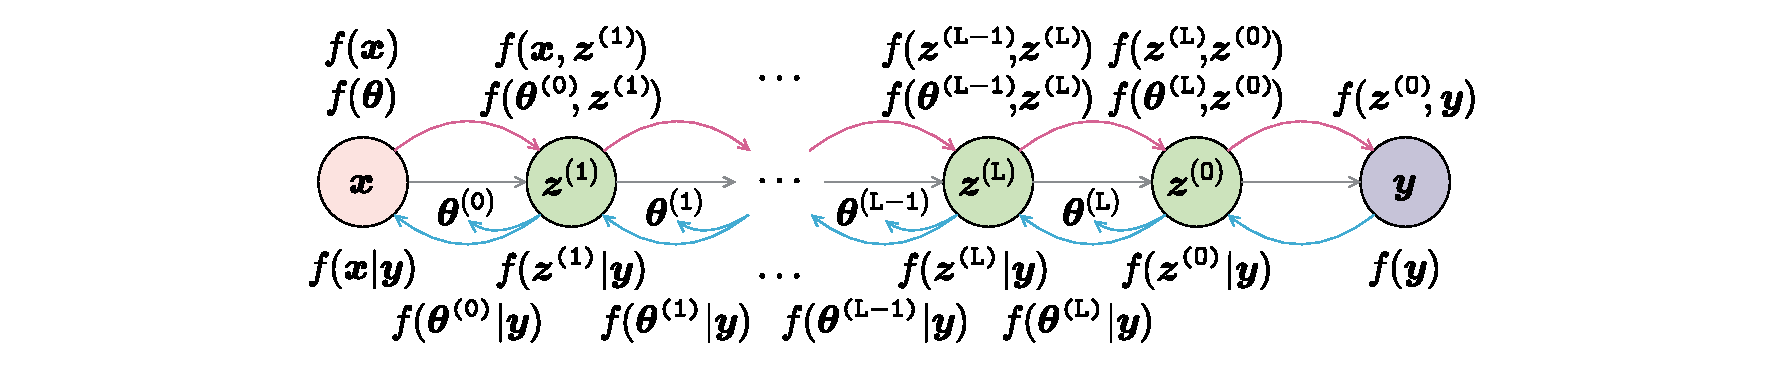
\includegraphics[width=\textwidth]{tagi.pdf}
    \caption{Graphic illustration of TAGI's forward and inference steps for a neural network architecture.}
    \label{fig:tagi}
\end{figure}
    \item \textbf{Development of a NumPy-Based Application:} We developed a NumPy-based application to replicate the regression toy example from the paper shown in \ref{fig:toy_example}. This implementation serves as a verification step to make sure that the formulation is identical with what is presented in the paper.
\begin{figure}[h]
    \centering
    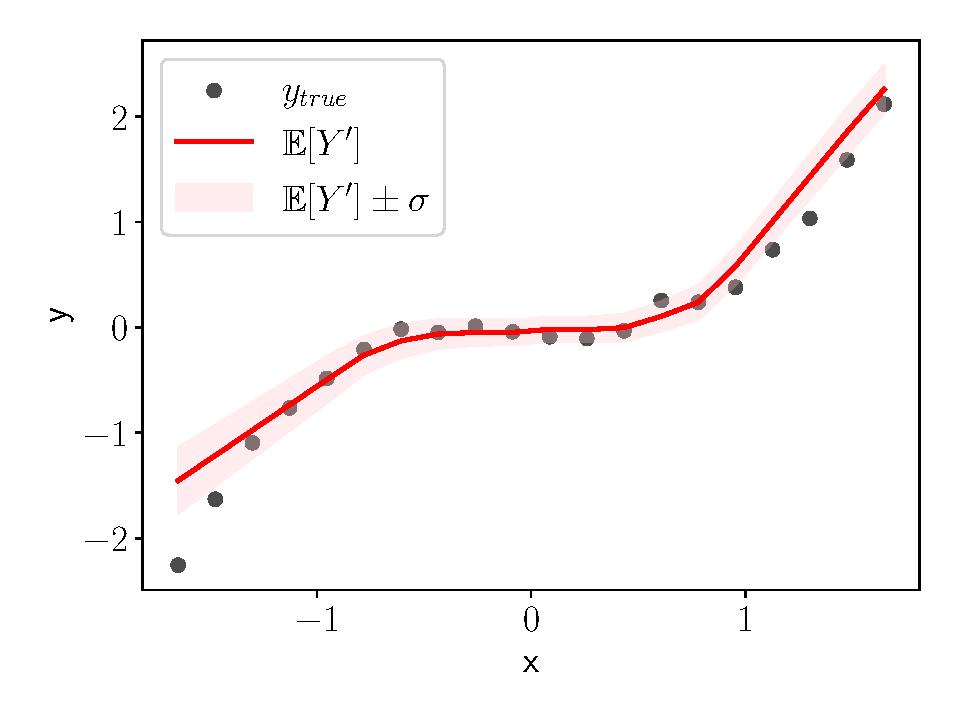
\includegraphics[width=0.4\textwidth]{toy_example.pdf}
    \caption{Obtained results on the replicated toy example.}
    \label{fig:toy_example}
\end{figure}
\end{itemize}

\subsection*{Implementing TAGI for Classification}
%Next, we are working on replicating the softmax formulation as prepared by the authors of the paper. This formulation enables a Gaussian approach to the softmax activation function, facilitating more efficient and scalable classification tasks.
We are currently working on implementing a probabilistic softmax activation function for classification tasks. However, as we will detail in the final report, the probabilistic softmax has shown poor performance in our experiments. To address this, we plan to implement an alternative activation function, called \textit{remax}, which offers better performance. In the remax function, the standard softmax operation $a_i = \frac{\exp(z_i)}{\sum \exp(\mathbf{z})}$ is replaced with $a_i = \frac{\text{mrelu}(z_i)}{\sum \text{mrelu}(\mathbf{z})}$ where \textit{mReLU} is a Gaussian-mixture ReLU. This implementation will be integrated into the \texttt{cuTAGI} \cite{cutagi2022} library to ensure optimal computational efficiency.


\subsection*{Comparing TAGI with Backpropagation}
%Finally, we have set up experiments using \texttt{pyTAGI} and \texttt{PyTorch} to evaluate both learning paradigms. This comparison aims to reveal the strengths and weaknesses of each approach. Our analysis includes: (1) Various Machine Learning Tasks: evaluating performance across different tasks to assess versatility. (2) Diverse Neural Network Architectures: testing on multiple architectures to determine scalability and adaptability. (3) Performance Metrics: comparing accuracy, convergence speed, and computational efficiency. (4) Robustness and Stability: analyzing how each method handles noisy data and avoids overfitting.
We will compare \texttt{pyTAGI} and \texttt{PyTorch} on a regression task (Boston Housing) and a classification task (MNIST) using the following setups:
\begin{itemize}
\item \textbf{Architectures:} FNN, CNN and ResNet.
\item \textbf{Configurations:} Different numbers of layers (1, 3, 5), neurons per layer (16 - 128), batch sizes (1, 8, 16, 256), batch and layer normalization.
\item \textbf{pyTorch-Specific:} Varying learning rates values (e.g., 1e-3, 1e-2, 0.1).
\item \textbf{pyTAGI-Specific:} Varying $\sigma_v$ values (e.g., 0.01, 0.05, 0.1, 0.2, 0.5, 1.0).
\item \textbf{Metrics:} Accuracy, convergence speed, and training efficiency.
\end{itemize}
The goal is to collect results under different setups to find optimal configurations and determine scenarios where pyTAGI outperforms PyTorch. This is in order to determine the advantages of PyTAGI compared to classical NNs.


\bibliographystyle{plain}
\bibliography{references}

\end{document}